\chapter{Literature Review}
% -_____________________________________________________________________________

\section{Goals And Methodology}
This project aims to find the

% -_____________________________________________________________________________

\section{Blockchain Basics}


\subsection{How it works}

Similar to a linked list, a blockchain is a series of 'blocks' containing some information, with each block linked to the block before, using deterministic cryptographic hashes. This forms an immutable chain of blocks holding hashed information that cannot be altered, known as the ledger, shown in \fref{Figure:BasicBlockchain}. Altering the information held in any block in this ledger invalidates the hashes of all the blocks after it. This is what makes blockchains resistant to data modification. Each participant in the network will be referred to as a node in this paper. Each node holds its personal copy of the transactions and hashed blocks and is responsible for spreading any new transaction information to the whole network.

\begin{figure}[h]
    \centering
    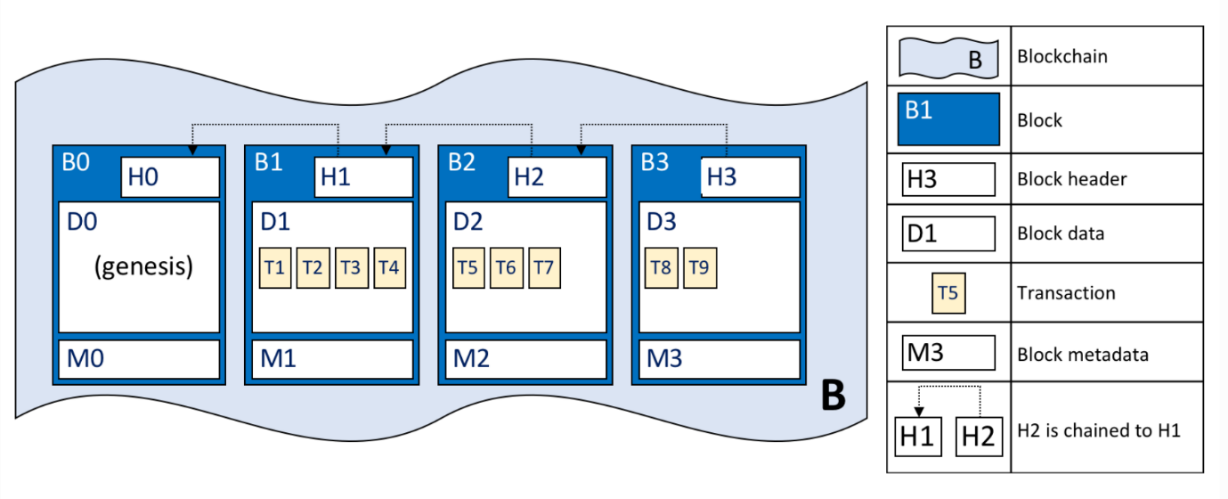
\includegraphics[width=13cm,center]{Figures/BlockchainStructure.png}
    \caption{The data structure underlying blockchain \cite{ADocumentation}}
    \label{Figure:BasicBlockchain}
\end{figure}

Blockchains remove the need for an intermediary between 2 parties involved in a transaction, such as a bank that controls the whole process. External authorities are not required to validate the authenticity and integrity of data. It is a decentralised form of immutable storage that serves as the single source of truth to all nodes on the network creating trust between anonymous actors.

There is a consensus protocol that varies from blockchain to blockchain. It describes how nodes validate and agree on adding new transactions to the ledger. These consensus mechanisms defend against a plethora of attacks that malicious nodes could attempt.




% -_____________________________________________________________________________

\subsection{Consensus in Blockchain Systems}
\url{https://vitalik.ca/general/2017/12/31/pos_faq.}
\url{https://vitalik.ca/general/2017/12/31/pos_faq.html#what-is-weak-subjectivity}


% -_____________________________________________________________________________

\subsection{Types Of Consensus}




% -_____________________________________________________________________________

\subsubsection{Proof-Of-Work}




% -_____________________________________________________________________________

\subsubsection{Proof-Of-Stake}





% -_____________________________________________________________________________

\subsection{Types Of Blockchains}



% -_____________________________________________________________________________

\subsubsection{Public Vs Private Vs Permissioned}


% -_____________________________________________________________________________

\section{Ethereum Basics}

***explain the whole of ethereum from an all inclusive perspective, inclusing like why gas exists, what it is, very simply. And teh Dapp ecosysm, and how eth is just a the bottom layer, why Eth exists basically.

***introduce what a blockchain is, basics

Nodes that communicate over a network following the 'ETH' protocol form the Ethereum network, also called the Ethereum 'mainnet'. These nodes contribute to maintaining and securing a globally agreed state of the Ethereum Virtual Machine (EVM). ***expand
The security of this network comes from a majority of nodes agreeing on the new change to the state of this EVM. In other words, agreeing on the next block to be permanently added to the blockchain ledger. Such nodes are paid in Ethereum's native cryptocurrency, \textbf{Ether (ETH)}, to run validator software that validates new blocks received over the peer-to-peer network.

***Introduce the need for consensus protocols

Ethereum is a permissionless blockchain. This means anyone can download the software and start interacting with the Ethereum blockchain. This interaction between a client and the Ethereum blockchain is enabled by the JSON RPC(Remote Procedure Call) API. When any user wants to complete a transaction with another user across the network, they:
\begin{enumerate}
    \item Need to specify the transaction amount
    \item Secure the transaction with their own private key
    \item Specify the tip they are willing to pay on top of the base transaction fees (both in 'gas' units) to incentivise a validator to validate and include their transaction in an upcoming block
\end{enumerate}

The ETH Execution client verifies the transaction request by checking things like whether the user has enough ETH to complete the transaction and if they have used the correct private key etc. \cite{EthereumEthereum.org}. 
This transaction request is then broadcasted to every other validator node over the execution layer 'gossip network'. Every validator adds this transaction to their local \textbf{'mempool'}. This is a collection of unverified transactions that are waiting to be processed and added to a new block.

In pre-merge PoW Ethereum, miners would have to compete with other miners to solve a computationally- complex problem in a brute-force manner, expending as much computational power as they could. The winner was chosen to be the block proposer for the next block added to the ledger, consequently receiving the rewards that come with it.

% -_____________________________________________________________________________
\subsection{"The Merge" - PoS Ethereum}

\url{https://blog.ethereum.org/2021/05/18/country-power-no-more}

"The Merge", also known as the "Paris Upgrade", happened on 15$\mathrm{^{th}}$ September 2022. The Ethereum Blockchain switched from the older Proof of Work (PoW) to the Proof-of-Stake (PoS) consensus protocol. It was coined 'the Merge' as the Beacon Chain (a testing network) was merged with the original Ethereum network. Both networks now operate simultaneously in layers. The older Ethereum chain is now known as the 'execution' layer (EL), now secured by the PoS 'consensus' layer (CL), formerly known as the Beacon Chain. 

The merge of the original chain with the Beacon Chain makes miners redundant. \textbf{Validator nodes} now secure the Ethereum network. 

\subsubsection{Full Nodes}
There is a popular mantra in blockchain, "Don't trust, verify" \cite{EthereumEthereum.org}. Following this altruistic mantra, running a Full Node allows a user to interact with the Ethereum Network in a trustless and self-sufficient manner. Everything can be checked and verified by your own node, removing the need to trust information from any other nodes in the network. 

Full Nodes need to run both an EL and CL client and must have  synchronised with the latest version of the blockchain in order to interact with the blockchain. 

\subsubsection{Validator Nodes}
To participate in the validation of transactions, Full Nodes must run an additional validator client and put 32 ETH at stake (currently equivalent to £45000) as collateral. Validator nodes are responsible for storing data, processing transactions and adding new blocks to the Ethereum blockchain permanently. 

Blocks are 'forged' by validators at a fixed tempo in PoS Ethereum. Every 12-second time \textbf{'slot'}, a pseudo-randomly selected validator gets to forge a new block and broadcast it to the rest of the network. Validators can choose which transactions in their mempool they will include in their next block. Validator client software executes these transactions locally, proposing a state change (such as a change in account balances). Once it completes enough transactions to fill up a block (there is a gas limit per block), it proposes this signed 'beacon' block to all other validators over the consensus layer (CL) network. This block is also wrapped in other information such as rewards, slashings, and attestations, which are discussed later.

32 time slots make up an \textbf{epoch}, usually around 6 minutes. For every slot, apart from selecting a block proposer (validator), a small committee of nodes is also randomly selected, whose votes determine whether the proposed block is valid or not. When these nodes receive the proposed block from the chosen validator, they pass it on to their Execution Layer Client (EL), where the block's data is verified. This includes ensuring the block corresponds to the correct slot, correct parent etc. Most importantly, the transactions in the block are re-executed to check that the proposed state changes are valid \cite{EthereumEthereum.org}. If the new block passes all checks, the nodes add it to their own local canonical blockchain. The one they believe to be the single source of truth. 

The algorithm judges each validator's actions and dishes out rewards and penalties at the end of each epoch accordingly. 

***Instead of sharding, explain attestations here, include a diagram \url{https://kb.beaconcha.in/attestation}

% \textbf{Sharding} \label{Sharding}
% One solution to increasing the number of transactions throughput on the network is sharding. It refers to splitting the entire Ethereum network into 64 portions called \textbf{shards} \cite{Buterin2020Annotated-spec/beacon-chain.mdEthereum/annotated-spec}. Each shard would contain its own independent state. It is an attempt at breaking up the blockchain into smaller parts no nodes are not responsible for processing or re-executing every single transaction broadcasted on the Ethereum network. Each shard is still connected to the main Ethereum chain cryptographically through merkle trees. \cite{EthereumEthereum.org} 


\textbf{Attestations}

Validators are expected to create, sign and then propagate their attestation to the rest of the network, every epoch. It aims to vote in favour or against the blocks proposed in a specific epoch. Attestations of the first and last block of the epoch are the most important as they help to retrieve each validator's view of the blockchain after each epoch. This information is combined to help the network reach consensus about which version of the blockchain to follow.

 ****explain why client diversity is important
 **** once you have a node running, its not automatically a validator node
****reasons its good for the network if more poeple run a node, with which come energy consumption
 
\paragraph{Staking ETH}

There are many different ways to stake ETH as a validator, as not everyone has access to or is prepared to lock up 32 ETH for an indefinite period. To get past this high barrier of entry, users can opt for solo staking, staking-as-a-service, pooled staking or centralised exchanges using 3$\mathrm{^{rd}}$ parties. 

Some of the risks that come with staking include the following:
 % ***shorten this section, kee relevant bits
 
\textbf{Slashing :}
This is when the algorithm destroys a portion of a validator's stake for behaving maliciously/ against the best interests of the network.

\textbf{Offline Penalty :}
If a validator goes offline for a number of days, they incur losses roughly equivalent to what they would have gained had they remained online. 

'The Merge' substituted Ethereum's security model's reliance on computational power to \textbf{economic power}, which are comparable in many ways. Malicious attackers need 51\% of the economic power of the entire Ethereum network instead of 51\% of the mining power for a successful attack. These severe economic punishments help to keep the network more secure than before while massively reducing the energy consumption of the network. 
 % -------
\newline \newline
Equally, there are many incentives to run a validator node. These include:

\textbf{Block Proposer Rewards :}
This is the reward for those validators chosen to propose the next block in a slot. When their block is finalised, they are rewarded with a substantial amount of ETH.



% -_____________________________________________________________________________
\subsection{Ethereum Key Concepts}

\subsubsection{Node Types}

Validator nodes are responsible for one of the two:
\begin{enumerate}
    \item Propose a new block by executing pending transactions from the mempool when randomly chosen as a block proposer for a slot
    \item Check blocks other validator nodes are proposing and attest to them by checking their validity and voting 
\end{enumerate}
As explained before, these nodes must stake 32 ETH in order to participate in securing the Ethereum network and earn rewards for adding blocks to the blockchain.

The version of the ledger stored by Full Nodes and validators is periodically pruned so that they don't hold the entire chain dating back to the Genesis block. \textbf{Archive Nodes} are a type of node that maintain an exact and complete copy of the entire blockchain dating back to the Genesis block. 

Apart from users looking to earn ETH or altruistic users wanting to secure the Ethereum network, not many users have the incentive to invest the time and resources to run a Full Node. This is why most users end up using centralised 3rd party hosted nodes. Client wallets like MetaMask and MyEtherWallet connect to a remote node in a non-cryptographically proven matter. New lighter node types, such as Light Nodes, were introduced to help make Ethereum accessible to more users, which in turn also makes the network more secure.

% \textbf{Light Nodes :}
% These are nodes that don't stake Ethereum. Instead, they are just used for accessing the network along with storing and processing the validation of the blocks within the network. These rely on full nodes as intermediaries to receive up-to-date information about the state of the blockchain. In essence, they are spectator nodes that constantly monitor the network and are witnesses that all activity complies with the rules.

% Because they are up-to-date nodes, they are allowed to interact with the Ethereum blockchain.  All they require is a simple installation of an ETH 2.0 node and a connection to the internet. This means the minimum requirements for the hardware required to run a light node is minimal and can be run on mobile devices.

% By design, they don't need to store or process the same amount of information that full nodes do. PoW light nodes only used download the headers of each block and were able to trace back. PoS light nodes also has to keep track of validators and their balances to stay on the chain with the most stake. This small amount of information allows light nodes to operate in a trust-minimised manner.


\subsubsection{Client Types and Synchronisation}

In the context of a blockchain, client software is software that connects users to each other in a peer-to-peer manner. Due to this cross-communication, these clients form a network where each client acts as a node. 

\textbf{Execution Layer Clients}

EL clients come in the form of community-maintained open-source software, formerly known as 'Eth 1' clients. Having a diverse share of client software being run on nodes participating in the network makes it more decentralised and reduces single points of failure.

Some popular EL clients include Geth, Nethermind, Besu and Erigon, written in languages such as Java, Go, and C\# \cite{EthereumEthereum.org}. 

\textbf{Consensus Layer Clients }

Following 'The Merge', CL clients, also known as 'Eth 2' clients, provide the security layer to the Ethereum network. This layer is responsible for the PoS consensus mechanism.

Some popular CL clients include Prysm, Lighthouse, Teku, Nimbus and Lodestar, written in languages such as Rust, Nim, Typescript and Go \cite{EthereumEthereum.org}. 

The latest network shares of each of these EL and CL clients can be found in \tref{Table:ClientShares} in \sref{Modelling}.

\textbf{Synchronisation} 

Synchronisation refers to a new node catching up to the latest version of the Ethereum Blockchain by retrieving the most up-to-date information. This is done by requesting data from peers. This data is cryptographically verified and used to build a local copy of the blockchain, treated as the single source of truth.

PoS Ethereum relies on the Consensus Layer for handling consensus logic and block propagation. Thus, synchronisation is a shared process between the EL and CL client. In order for the EL client to start verifying and syncing a local copy of the blockchain, the CL client has to download the block header. Only when the CL client provides the EL client with a header to use as a synching target can it cryptographically verify the chain of blocks being synced is valid. After this chain of block headers has been formed and validated, the rest of the blocks' information is downloaded \cite{2022DeveloperGo-ethereum}. This is the step that often takes the longest.

Many syncing modes exist, such as Full, Snap, Fast and Light Sync.

\textbf{Full Sync }independently verifies the block provenance by re-executing the transactions starting at the Genesis Block. However, only the latest 128 blocks are actually stored in the Full Node, along with a few checkpoints representing older blocks. 

\textbf{Snap Sync }was developed by Geth developers(the prevailing EL client). It works similarly to a Full Sync, except it starts at a much more recent checkpoint to start its verification up to the front of the chain \cite{2022DeveloperGo-ethereum}.

Synchronisation times vary depending on the client software chosen as well the node's hardware configuration. It is not uncommon for syncing times to range between 12 hours and 6 days.
% -_____________________________________________________________________________



\section{Energy Consumption And Carbon Emissions of Blockchain Systems}



% -_____________________________________________________________________________

\subsection{Papers On Carbon Emissions of Blockchain Systems}


% -_____________________________________________________________________________

\subsection{Papers On Modelling Energy Usage Of Blockchain Systems}


% -_____________________________________________________________________________

\subsubsection{Experimental Papers}



% -_____________________________________________________________________________

\subsubsection{Mathematical Papers}



\subsection{ Existing models }
\label{LitRevExistingModels}
\textbf{The CCRI Merge Paper } \cite{CryptoCarbonRatingsInstitute2022TheNetwork}

Assumptions this paper makes:
\begin{itemize}
    \item Assumes the syncing energy of each node will skew energy averages, so ignores node bootstrapping energy usage during the sync phase.
    
    \item They run many full nodes with different combinations of execution and consensus layer clients. However, they did not then proceed further and run a validator node due to the high economic barrier of entry (staking 32 ETH). They claim the energy usage of turning it into a validator would be negligible.
    
    \item Did not consider light nodes and archive nodes, presumably because of the assumption that their energy usage will be negligible as well as the lack of support of light nodes at the time.

    \item Type of power supply and mainboard was not mentioned. This is important to the estimation as power efficiencies cause more power to be drawn from the grid than the amount that is utilised by a computer.
\end{itemize}

% -_____________________________________________________________________________


% Quick intro on AVX operations, what is TDP and why that is the upper limit of CPU power consumption
AVX instructions enable the processor to perform multiple floating-point operations at the same time, resulting in faster computation and improved performance. \cite{Schuchart2016TheScale}

% ______________________________________________________________________________


\section{Key Points Covered}
